% !TEX root = ../ArticleTemplate.tex
%%%%%%%%%%%%%%%%%%%%%%%%%%%%%%%%%%%%%%%%%%%%%%%%%%%%%%%%%%%%%%%%%%%%%%%%%%%%%%%%%%
\section{PGF and Tikzpicture}
\subsection{Boxes}
\begin{verbatim}
\boxed{Example}
\end{verbatim}
\[\boxed{Example}\]

\begin{verbatim}
	\begin{Intro}[colbacktitle=red]{Titolo}{Testo}\end{Intro}
\end{verbatim}

\paragraph*{}
Other alternatives are given by the environments listed in Section \ref{ChapIntro}.
%%%%%%%%%%%%%%%%%%%%%%%%%%%%%%%%%%%%%%%%%%%%%%%%%%%%%%




\subsection{PGF (see also the manual of the package "pgfplots" on \texorpdfstring{\url{ctan.org}}{ctan.org})}

\begin{center}
\fbox{\parbox{.8\textwidth}{This section presents only a few examples. Due to Overleaf's reduced compilation time in the free version, I don't include the images generated by the code shown in verbatim.}}
\end{center}

\newpage
\begin{verbatim}
\begin{figure}[ht]
\centering
\begin{tikzpicture}[scale=1.75]
    \begin{axis}[xmin=-0.5, xmax=5, ymin=-0.5,
	    axis equal, xtick=data, ytick=data, grid=major]
        
        \addplot[only marks] coordinates {(4,1) (3,1) (1.5,3)};
   	    
        \addplot[mesh, domain=0:2.5, tick=\empty]
            {(x-.5)^2}  node [pos=.25, pin=0.4:$p$] {$\bullet$}
   	                    node [pos=.6, sloped, xshift=.05cm, yshift=-.2cm]
                                {\scriptsize $y=(x-\nicefrac12)^2$};
    \end{axis}
\end{tikzpicture}\noindent\hspace{2cm}
\caption{Points and graphs}
\end{figure}
\end{verbatim}

%%%%%%%%%%%%%%%%%%%%%%%%%%%%%%%%%%%





\newpage
\begin{verbatim}
\begin{figure}[ht]
\centering
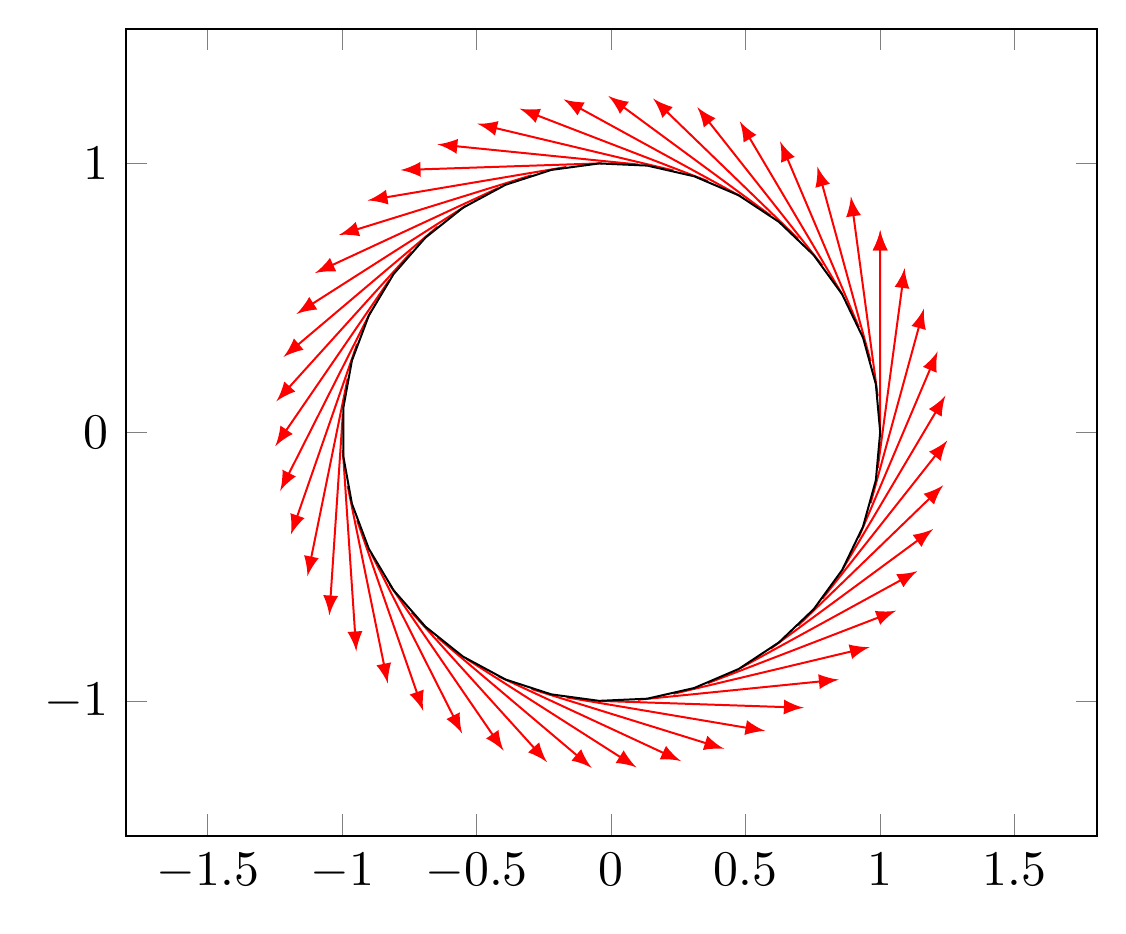
\begin{tikzpicture}[scale=1.8]
    \begin{axis}[xmin=-1.5, xmax=1.5, ymin=-1.5, ymax=1.5, axis equal]
    
        \addplot[samples=48, domain=0:2*pi, -latex, variable=\t,
            quiver={u={-sin(deg(t))},
                    v={cos(deg(t))},
                    scale arrows=0.75,
                    colored=red}]
                ({cos(deg(t))}, {sin(deg(t))});
       
        \addplot[samples=36, domain=0:2*pi]
            ({cos(deg(x))}, {sin(deg(x))});
    \end{axis}
\end{tikzpicture}
\caption{Parametrizations}
\end{figure}
\end{verbatim}
%%%%%%%%%%%%%%%%%%%%%%%%%%%%%%%%%%%





\newpage
\begin{verbatim}
\begin{figure}[ht]
\centering
\begin{tikzpicture}[scale=1.5]
    \begin{axis}[xmin=-5, xmax=5, ymin=-28, axis equal]
        
        \addplot[samples=24, domain=0:2*pi, dashed, data cs=polar,
        top color=Blues-I, bottom color=Blues-B] (deg(x),30);
        
        \addplot[name path=Y, samples=24, domain=0:2*pi, dashed, 
        data cs=polar] (deg(x),30);
        
        \addplot[GnBu-M, name path=X, domain=0:360, samples=36, smooth,
        data cs=polar] (x, {30-8*sin(3*x)});
        
        \addplot[green] fill between[of=Y and X];
        
        \addplot [samples=36,domain=0:30, dashed, data cs=cart]
        {.025*x^2} node [pos=1.1] {Node};
        
        \addplot[mark=oplus, only marks] coordinates {(0,0)};
        \node[pin=120:{Pin}] at (0,0) {};
    \end{axis}
\end{tikzpicture}
\caption{Nodes and filling}
\end{figure}
\end{verbatim}

%%%%%%%%%%%%%%%%%%%%%%%%%%%%%%%%%%%





\newpage
\begin{verbatim}
\begin{figure}[ht]
\centering
\begin{tikzpicture}[scale=1.75]
    \begin{axis}[xmin=-1, xmax=2, ymin=-3.5, ymax=1, axis equal=false]

        \addplot[red, patch type sampling, patch type= cubic spline,
        domain=0:2, smooth]{ln(x)};
        
        \draw (0,0) .. controls (1,-1.2) and (1,1) .. (2,1);
   \end{axis}
\end{tikzpicture}
\caption{Interpolation and paths}
\end{figure}
\end{verbatim}
%%%%%%%%%%%%%%%%%%%%%%%%%%%%%%%%%%%





\newpage
\begin{verbatim}
\begin{figure}[ht]
\centering
\begin{tikzpicture}[scale=1.75]
    \begin{axis}[colormap/PuBu, samples=10, domain=-4:4, y domain=-4:4,
    xmin=-4, xmax=4, ymin=-4, ymax=4, enlargelimits=false]
    
    \addplot3[surf, samples=18, samples y=36]{x^2+y^2-1};
\end{axis}
\end{tikzpicture}	
\caption{3D Surfaces}
\end{figure}
\end{verbatim}
%%%%%%%%%%%%%%%%%%%%%%%%%%%%%%%%%%%





\newpage
\begin{verbatim}
\begin{figure}[ht]
\centering
\begin{tikzpicture}[spy using outlines={}]
    \begin{axis}[xmin=-1, xmax=6, ymin=0, ymax=1,
    axis equal=false, grid=major, xtick=data, ytick=data,
    every axis plot post/.append style={thick}]

        \addplot[line join=round, green]
            coordinates {(1, 0) (1,.75) (3, 0.9) (4, .75) (5, 0.8)};
            
        \addplot[line join=bevel, blue]
            coordinates {(0, 0) (1, 0.4) (3, 0.2) (4, 1) (5, 0.9)};

        \coordinate (spypoint)     at (1,.4);
        
        \coordinate (magnifyglass) at (-2,.25);
\end{axis}
\spy[blue, size=1.5cm, circle, magnification=5, connect spies]
    on (spypoint) in node[fill=white]
                  at (magnifyglass);
\end{tikzpicture}	
\caption{Spy}
\end{figure}
\end{verbatim}

%%%%%%%%%%%%%%%%%%%%%%%%%%%%%%%%%%%





\newpage
\begin{verbatim}
\begin{figure}[ht]
\centering
\begin{tikzpicture}[scale=1.75]
	\begin{axis}[xmin=0, xmax=3.5, ymin=0, ymax=5]
	   
       \draw [name path=A] (2,3) ellipse (1.5 and 1.25);
	   
       \draw [name path=B] (1.5,1.5) rectangle (3,5);
       
       \fill [red, opacity=.5, name intersections={of=A and B}]
            (intersection-1) circle (2pt) node[above right] {1}
            (intersection-2) circle (2pt) node[above left] {2} 
            (intersection-3) circle (2pt) node[below left] {3} 
            (intersection-4) circle (2pt) node[below right] {4};
	\end{axis}
\end{tikzpicture}
\caption{Intersections}
\end{figure}
\end{verbatim}

%%%%%%%%%%%%%%%%%%%%%%%%%%%%%%%%%%%





\newpage
\begin{verbatim}
\begin{figure}[ht]
\centering
\tdplotsetmaincoords{70}{135}
\begin{tikzpicture}[scale=3, tdplot_main_coords]
    
    \tdplotsphericalsurfaceplot[parametricfill]{36}{36}
        {sqrt(15/2)*sin(\tdplottheta)*cos(\tdplottheta)}
        {black!10}{\tdplotphi};

    {\draw[color=black,thick,->] (0,0,0) -- (2,0,0) 
        node[anchor=north east]{$x$};}

    {\draw[color=black,thick,->] (0,0,0) -- (0,2,0) 
        node[anchor=north west]{$y$};}
    
    {\draw[color=black,thick,->] (0,0,0) -- (0,0,2) 
        node[anchor=south]{$z$};}
\end{tikzpicture}
\caption{Tikz-3dplot}
\end{figure}
\end{verbatim}

\newpage